\chapter{Overview of an optical SISO system}
\label{chapter:siso}
\thispagestyle{myheadings}
An optical SISO link can be established between a single transmitting element and a single receiving element. This chapter outlines coordinate systems used for analysis in this work. An overview of common optical terminology and an optical signal chain is then provided. An outline of the SISO channel model is then provided along with a mathematical representation of different components involved in the system. An overview of frequently considered optical SISO channel modulation techniques is then provided. 

% -------------------------------------
% SECTION: Coordinate System
% -------------------------------------
\section{Coordinate Systems}
\label{sec:coordinate}
\graphicspath{{_Intro/Figures/}}

\begin{figure}[!b]
	\centering
		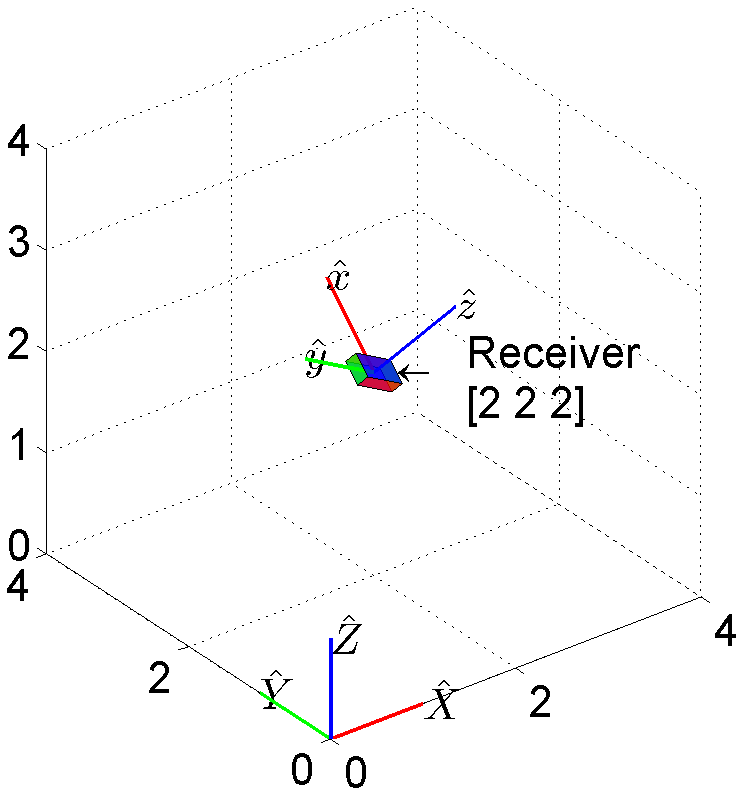
\includegraphics[width=3in]{figRcvrOrientation2.png}
	\caption{Illustration of the coordinate systems used}
	\label{fig:RcvrCoord}
\end{figure}

\figurename{ \ref{fig:RcvrCoord}} illustrates coordinate systems used in the analysis. [$\hat{\bf{X}}$ $\hat{\bf{Y}}$ $\hat{\bf{Z}}$] and [$\hat{\bf{x}}$ $\hat{\bf{y}}$ $\hat{\bf{z}}$] are the basis vectors for the GCS and the RCS. A corner of the room is the origin of the GCS while the center of the aperture of the receiver is set as the origin of RCS. The receiver's basis vectors are assumed always parallel to the length, width and surface normal of the sensor. 

Let [$x_{tx}$ $y_{tx}$ $z_{tx}$] be the location of centroid ($C_{tx}$) of the illumination surface of the transmitter and [$x_{rx}$ $y_{rx}$ $z_{rx}$] be the location of the centroid of the receiver concentrator surface in the GCS. The optical axis is then defined by ${\bf{d}}$ and the vertical distance between the transmitter and receiver is given by ${\bf{d}^{z}}$.

\begin{equation}
\label{eqOpAxis}
	{\bf{d}}=\vectthree{x_{tx}}{y_{tx}}{z_{tx}} - \vectthree{x_{rx}}{y_{rx}}{z_{rx}}
\end{equation}

\begin{equation}
\label{eqTxRxDist}
	{\bf{d}^{z}}=({\bf{d}}.{\hat{\bf{z}}}){\hat{\bf{z}}}
\end{equation}

% -------------------------------------
% SECTION: Outline
% -------------------------------------
\section{The Optical Downlink}
\label{sec:outline}
\graphicspath{{_Intro/Figures/}}

\subsection{Common terminology}
\label{subsec:outlineTerminology}
This sub--section outlines optical terminology used in the rest of the text.
\subsubsection{Radiant flux}
\label{subsubsec:radiantFlux}
Radiant flux is the amount of radiant energy emitted per unit time by an optical source. Let $P(\lambda)$ be the SPD under consideration. The radiant flux $\Phi_{W}$ corresponding to the SPD is given by 
\begin{equation}
	\Phi_{W} = \int\limits_{\lambda_{min}}^{\lambda_{max}}P(\lambda)d\lambda
	\label{eqRadiantFlux}
\end{equation}
(Units: W).

\subsubsection{Radiant intensity}
\label{subsubsec:radiantIntensity}
Radiant intensity is the amount of radiant flux emitted per unit solid angle by an optical source. (Units: W/sr)

\subsubsection{Irradiance}
\label{subsubsec:irradiance}
Irradiance is the amount of radiant flux received by a surface/device per unit area. (Units: W/m$^{2}$)

\subsubsection{Luminous flux}
\label{subsubsec:luminousFlux}
Luminous flux is the amount of luminous energy emitted per unit time by an optical source. Let $P(\lambda)$ be the SPD under consideration. The luminous flux $\Phi_{lm}$ corresponding to the SPD is given by \cite{gru08b}
\begin{equation}
	\Phi_{lm} = 683\int\limits_{380\text{ nm}}^{780\text{ nm}}P(\lambda)V(\lambda)d\lambda
	\label{eqLuminousFlux}
\end{equation}
where $V(\lambda)$ is the eye sensitivity function. (Units: lm).

\subsubsection{Luminous intensity}
\label{subsubsec:luminousIntensity}
Luminous intensity is the amount of luminous flux emitted per unit solid angle by an optical source. (Units: lm/sr)

\subsubsection{Illuminance}
\label{subsubsec:illuminance}
Illuminance is the amount of luminous flux received by a surface/device per unit area. (Units: lm/m$^{2}$)


\subsection{The optical downlink}
\label{subsec:outlineDownlink}

The OWC system operates under the hybrid wireless model paradigm using the visible light communication (VLC) channel as the high capacity downlink and another medium for the uplink. This seems to be the accepted model and a reasonable assumption \cite{rah15a}. \figurename{ \ref{fig:VLCdownBD}} illustrates a block diagram for a typical VLC downlink. 

\subsubsection{Data source}
\label{subsubsec:outlineSource}
The source is an entity that, while performing its tasks, produces or replicates information that needs to be communicated to another entity. 

\subsubsection{Coder}
\label{subsubsec:outlineCoder}
The coder assigns a binary bit sequence to the information from the source. In this process, it may introduce redundancy to reduce the effect of noise and interference in the channel. 

\subsubsection{Illumination state}
\label{subsubsec:outlineIllumination}
The illumination state sets the average output flux and the spectral power distribution (SPD) to be produced by luminaire(s). This is a result of a number of factors such as (a) requested illumination level by users in the space (b) optimal energy usage (c) output of `smart' applications such as circadian control, etc...

\begin{figure}[!t]
	\centering
		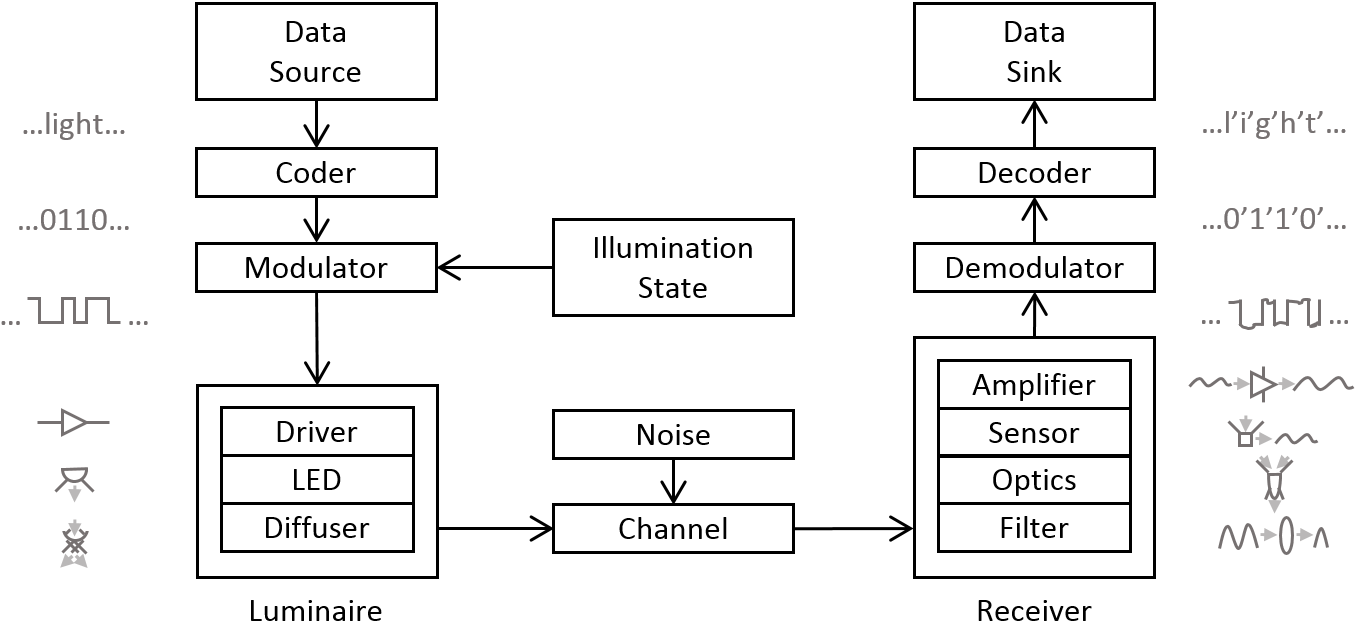
\includegraphics[width=6in]{vlcdownlinkBD.png}
	\caption{OWC downlink block diagram}
	\label{fig:VLCdownBD}
\end{figure}

\subsubsection{Modulator}
\label{subsubsec:outlineModulator}
The modulator, with the knowledge of requested flux, maps and converts the bit sequence into a corresponding waveform that drives the luminaire. The frequency of visible light is in the range of about 380 THz -- 780 THz. The current state-of-art electronics cannot sample and process signals at that high speeds. Thus traditional modulation schemes which vary the amplitude, frequency or phase of the waveforms within the RF spectrum cannot be directly implemented within the visible spectrum. Instead, the average power (a.k.a flux/intensity) of the visible waveforms are modulated to transmit data. Optical sensors like photodiodes (PD) produce output current proportional to the intensity of the incident radiation and not the waveform of the radiation itself. This signaling scheme is known as IM/DD. All optical modulation techniques are implemented in conjunction with IM/DD. This method introduces unique constraints that differentiate optical modulation techniques from RF modulation techniques.

\subsubsection{Luminaire/Transmitter}
\label{subsubsec:outlineLuminaire}
The luminaire is composed of a driver, LEDs and diffuser optics. A simple LED driver is a trans--conductance amplifier whose input is the waveform produced by the modulator. The corresponding output current drives the LED which in turn generates light. A luminaire is made up of number of phosphor converted white LEDs or different narrow--band devices which produce different colors. A phosphor converted white LED is made by coating a blue LED with yellow phosphor. The blue light excites the yellow phosphor and together they produce white light. The diffuser scatters the light produced by the LED(s) to mix the different colors and output a relatively homogenous, glare--free light which makes the luminous surface appear softer and more pleasing to the eye. Different diffuser front ends generate different sizes of cones of emission. The most common emission pattern is the Lambertian pattern. 

\subsubsection{Channel}
\label{subsubsec:outlineChannel}
The channel is the medium through which information flows. It is made up of all the paths traveled by the light rays between the luminaire and the receiver. Depending on the number of transmitters, colors or number of receiving elements, the channel can be configured into a various single/multiple input single/multiple output configurations. For the OWC downlink, the indoor space acts as the channel. In addition to the line-of-sight (LOS) path from the luminaire to the receiver, various reflected rays of light propagating over different path lengths may be incident on the receiver. In an RF system, such multi--paths cause inter-symbol-interference (ISI) that needs to be resolved for. In the indoor OWC system, due to poor reflectivity off various walls and directionality of receiving optics, optical signals propagating over such multi--paths have been shown to be heavily attenuated when incident on the active element of the receiver. In addition, difference in path lengths between LOS and non-LOS (NLOS) propagation within indoor spaces is very small. This produces a small delay spread which is insignificant when compared to frequency of intensity modulation.

\subsubsection{Receiver}
\label{subsubsec:outlineReceiver}
A receiver is made up of an optical filter, refractive optics, an optical sensor like PD and an amplifier. Some high speed systems transmit data over a small range of wavelengths (ex blue (400 nm -- 500 nm)) while the entire visible spectrum is used for illumination. In such cases, a blue filter is used to remove noise from parts of the optical spectrum that do not carry any information. For wavelength division multiplexed (WDM) systems where data is transmitted independently over different parts of the spectrum, multiple non--overlapping filters are used to decorrelate the different streams of information. For single pixel receivers, concentrator optics are used to increase the effective area of the sensor while keeping its capacitance at a minimum. A number of single pixel receivers can be configured in a matrix pattern to realize a non--imaging multiple element receiver. For imaging receivers, imaging optics are used to help decorrelate the multiple channels. Sensor devices such as p-i-n junction photodiode (PIN-PD), avalanche photodiode (APD) or complementary metal oxide semiconductor (CMOS) active pixel devices generate an electrical signal proportional to radiant flux incident on the sensor. This electrical signal is amplified and conditioned before it is processed to recover transmitted information. Randomness in photon arrival and sensing gives rise to shot noise within the system. Amplifiers such as trans--impedance amplifiers (TIA) introduce thermal noise into the system. This noise then distorts the signal waveform and can cause errors in information recovery.

\subsubsection{Demodulator}
\label{subsubsec:outlineDemodulator}
With prior knowledge of the modulation scheme implemented, the demodulator makes an intelligent estimate of the transmitted signal waveform. After recovering the transmitted waveform, it de--maps it to recover the transmitted bit sequence. Significant noise that is not orthogonal to the signal waveform can introduce errors in the demodulated sequence.

\subsubsection{Decoder}
\label{subsubsec:outlineDecoder}
The decoder, with prior knowledge of the coding scheme implemented, tries to recover the transmitted information from the bit stream. Redundancy introduced in the coded data can help the decoder to detect and rectify errors.

\subsubsection{Data sink}
\label{subsubsec:outlineSink}
Ideally, the data sink is the entity to which the information was transmitted to. 


% -------------------------------------
% SECTION: SISO Channel
% -------------------------------------
\section{Optical SISO channel}
\label{sec:sisoChannel}
\graphicspath{{_SISO/Figures/}}

A SISO VLC link can be established between a single luminaire broadcasting information over optical spectrum  and a single receiver that can generate an electrical signal proportional to incident optical radiation. Let the radiant flux emitted by the transmitter be represented by $x$. Intensity modulation imposes a non--negativity constraint ($x\geq$ 0) on the transmitted signal. The emitted radiant flux also provides illumination. Let $P_{\text{avg}}$ be the average transmitted radiant flux to maintain user requested illumination levels. Thus mean of transmitted signal must equal $P_{\text{avg}}$.

The transmitted flux propagates through the indoor space and traverses over different paths arriving at the receiver. The received flux can be expressed as a convolution of the channel impulse response and transmitted flux waveform. Under the `luminaire as a transmitter' model, the LOS component of the received flux is dominant over the NLOS component. In addition to free space path losses, the NLOS component of the received flux undergoes additional attenuation due to non--ideal reflectivity of the walls. The delay spread for the indoor channel is small when compared to frequency of intensity modulation. Under these circumstances, the channel can be treated as a LOS channel and the channel impulse response can be represented by a single tap with gain $h$. 

At the receiver, additive noise independent of the signal is added to the received signal and represented by $w$. Let the total received signal and noise be represented by $y$. The SISO channel can then be modeled as in Eq. \eqref{eqSisoChannel}.
\begin{equation}
	\label{eqSisoChannel}
	y = hx + w
\end{equation}

The channel gain is a function of the radiant intensity of emitted flux, the free space square path loss, optical gains at receiver and receiver sensor responsivity. Let the radiant intensity emitted by the transmitter at any angle $\phi$ subtended between the transmitter surface normal and the optical axis be given by $L(\phi)$. Radiant intensity of a Lambertian transmitter of order $m$ is given by
\begin{equation}
	\label{eqLambertian}
	L(\phi) = \twopartdef{{\frac{(m+1)}{2\pi}}cos^{m}(\phi)}{-\pi/2\leq\phi\leq\pi/2}{0}{\mbox{ else}}
\end{equation}

The SISO receiver optics comprises of an optical concentrator. Incorporating a concentrator helps increase the effective area of the sensor. This enables the receiver to incorporate a sensor with smaller dimensions thus reducing its capacitance and enabling a higher receiver bandwidth. Additionally sensor with smaller dimensions enables a compact form factor which can then enable its integration within portable devices. Let $\psi$ be the angle between the receiver surface normal ($\hat{\bf{z}}$) and the optical axis (\vm{d}). Let $\eta$ be the refractive index of the material of the concentrator and $\psi_{\text{c}}$ be the field of view of the concentrator. Then the optical concentrator gain is given by
\begin{equation}
	\label{eqOpGain}
	G(\psi) = \twopartdef{\frac{\eta^{2}}{sin^{2}(\psi_{\text{c}})}} {0\leq\psi\leq\psi_{\text{c}}\leq\frac{\pi}{2}}{0}{\psi>\psi_{\text{c}}}
\end{equation}

Let $S(\lambda)$ be the normalized SPD of the normalized emitted radiant flux such that area under curve is 1 W. Let $R(\lambda)$ be the responsivity of the PD. An optical filter can be incorporated within the receiver to provide selectivity to wavelengths of interest and reject unwanted optical radiation thus reducing noise. Depending on construction of optical filter, its transmittance is a function of angle of incidence and wavelength of radiation. Let the transmittance of the filter be given by $T(\psi,\lambda)$. Thus the effective responsivity of the receiver including the transmission and gains from all optical components is given by 
\begin{equation}
	\label{eqReff}
	R_{\text{e}}(\psi) = G(\psi)\int^{\lambda_{\text{max}}}_{\lambda_{\text{min}}}S(\lambda)T(\psi,\lambda)R(\lambda)d\lambda
\end{equation}
where $\lambda_{\text{min}}$ to $\lambda_{\text{max}}$ span all the wavelengths of interest.

Let $A$ be the active area of the PD. The overall channel gain $h$ is a function of the parameters discussed above and is then given by
\begin{equation}
	\label{eqChGain}
	%h = L(\phi)\frac{A}{||{\bf{d}^{z}}||^{2}}cos(\psi)R_{\text{e}}(\psi) THIS IS WRONG 
	h = L(\phi)\frac{A}{||{\bf{d}}||^{2}}cos(\psi)R_{\text{e}}(\psi)
\end{equation}

Average flux incident on a PD introduces shot noise within the optical-to-electrical conversion process. In a typical SISO VLC link, shot noise from ambient illumination dominates over that from signal \cite{bar94a}. Let $q$ be the charge of an electron. Worst cast shot noise current density from isotropic ambient radiant flux $P_{\text{a}}(\lambda)$ is then given by
\begin{align}
	\sigma_{\text{sh}}^{2} &= 2q<I> \label{eqNshotGen}\\
	\sigma_{\text{sh}}^{2} &= \frac{2qAG(\psi_{\text{c}})}{\psi_{\text{c}}}\int_{\lambda_{\text{min}}}^{\lambda_{\text{max}}}\int_{0}^{\psi_{\text{c}}}P_{\text{a}}(\lambda)R(\lambda)T(\psi,\lambda)d\psi d\lambda 	  \label{eqNshot}
\end{align}
$<I>$ is the average current. Statistics of shot noise are typically Poisson in nature. For a large mean, a Poisson random variable can be approximated by a normal distribution with same variance. Thus, for the optical channel, shot noise is assumed to be distributed normally with variance $\sigma_{\text{sh}}^{2}$.

The TIA is generally the first current to voltage amplifier stage after the PD. In the absence of significant ambient illumination, the TIA noise is the dominant source of noise \cite{kah97a}. The thermal noise from the TIA is considered as the dominant electronic noise component. It is typically additive, white and Gaussian and its noise current density is given by \cite{kah97a},
\begin{equation}
	\label{eqNpa}
	\sigma_{\text{th}}^{2} = \frac{4kT}{R_{\text{f}}}
\end{equation}
where $k$ is the Boltzmann's constant, $T$ is the absolute temperature and $R_{\text{f}}$ is the feedback resistance of the TIA.
% 5pa/rt(Hz)

Thus the total noise current density can be computed from the shot noise current density and thermal noise current density. It is modeled as additive, white and Gaussian and its variance is given by 
\begin{equation}
	\label{eqNoise}
	\sigma_{\text{n}}^{2} = \sigma_{\text{sh}}^{2} + \sigma_{\text{th}}^{2}
\end{equation}

While $P_{\text{avg}}$ is the average transmitted radiant flux and let $B$ be the signal bandwidth. Using the parameters described above the SISO channel's SNR can be defined by Eq. \eqref{eqSisoSNR}.
\begin{equation}
	\label{eqSisoSNR}
	\text{SNR} \triangleq \frac{(hP_{\text{avg}})^{2}}{\sigma_{\text{n}}^{2}B}
\end{equation}
%Using Shannon's capacity formula for a AWGN baseband channel with a transmitter constrained to power $K$ independent of illumination and bandwidth $B$, the upper bound on capacity of the SISO VLC channel is given by \cite{sha48a}
%\begin{equation}
	%\label{eqSisoCap}
	%C_{SISO} < log_{2}\left(1 + \frac{h^{2}K}{\sigma_{SISO}^{2}B}\right)
	%%C_{SISO} = log_{2}(1 + SNR_{SISO})
%\end{equation}

%\footnotetext{An LED modulating at B Hz generates intensity signals band-limited in [-B B] and has signal bandwidth of 2B Hz}

% -------------------------------------
% SECTION: Modulation
% -------------------------------------
\section{Modulation Techniques}
\label{sec:sisoModulation}
\graphicspath{{_SISO/Figures/}}

The optical carriers span the electromagnetic spectrum within 380 THz -- 780 THz range. Lack of adequate electronics for passband transmission or reception at such high frequency ranges makes it impractical to implement coherent signaling schemes. However, it is possible to vary the intensity of such spectrum at the transmitter and detect it directly by optical flux to electrical signal conversion at the receiver. Thus, modulation techniques are implemented in conjunction with IM/DD to transfer information using the optical spectrum. A number of different modulation techniques have been studied for RF wireless communications. Some of those have been adapted for OWC due to the unique constraints of the optical channel. This section provides a summary of the more popular SISO modulation techniques.

\subsection{On-Off Keying}
\label{subsec:sisoModulationOOK}
\begin{figure}[t]
	\centering
		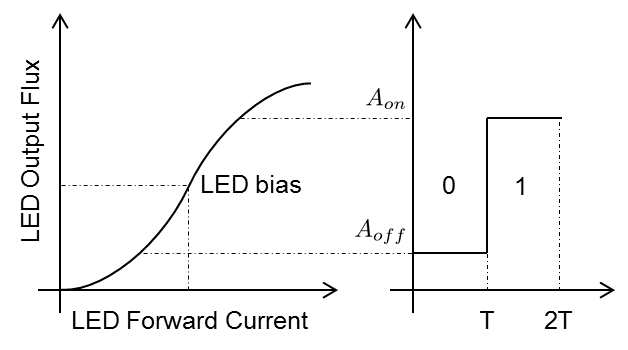
\includegraphics[trim={0in 0in 0in 0in}, clip=false, width=3.5in]{Signal_OOK.png}
		\caption{OOK signals.}
		\label{fig:sisoSigOOK}
\end{figure}
As the name suggests, OOK transmits information in the form of presence (on) or absence (off) of light. It is typically implemented under the NRZ model. To transmit bit `0', the transmitter drives all LEDs at a low intensity level and to transmit bit `1', it drives them all to a high intensity level. The on and off intensity levels can be set to achieve a desired average illumination level. \figurename{ \ref{fig:sisoSigOOK}} illustrates the OOK signal waveforms. $A_{off}$ is the low intensity radiant flux and $A_{on}$ is the high intensity radiant flux emitted by the LEDs at the off and on levels. If $p$ is the probability of transmitting bit `1', the average transmitted flux given by $A_{avg} = (1-p)A_{off} + pA_{on}$ is used to provide illumination whereas flux $A_{com} = p(A_{on}-A_{off})$ is used for communication. OOK-NRZ has a spectral efficiency of 2 bits/Hz. References \cite{kom04a,vuc09b} have demonstrated feasibility of OWC in indoor spaces while providing illumination using OOK.


\subsection{Pulse Amplitude Modulation}
\label{subsec:sisoModulationPAM}
\begin{figure}[t]
	\centering
		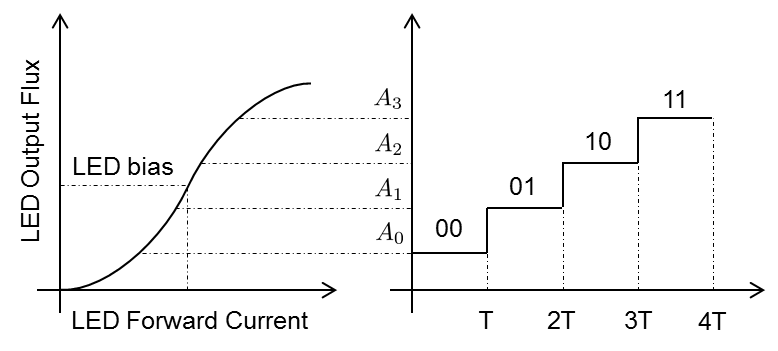
\includegraphics[trim={0in 0in 0in 0in}, clip=false, width=4.5in]{Signal_4PAM.png}
		\caption{4-PAM signals.}
		\label{fig:sisoSig4PAM}
\end{figure}
$M$-ary PAM can transfer information by varying the amplitude of each transmitted pulse. $m$=log$^{ }_{2}(M)$ bits to transmit are mapped to one out of $M$ possible pulse amplitudes. To transmit $m$ bits, the transmitter then drives all LEDs to emit radiant flux corresponding to the mapped amplitude. Let $A_{lo}$ be the lowest pulse amplitude and $A_{hi}$ be the highest pulse amplitude, then the $M$ different amplitude levels are given by $A_{i} = A_{lo} + i\times(A_{hi}-A_{lo})(M-1); 0\leq i<M$. For equi-probable bits, flux given by $A_{avg} = (A_{lo} + A_{hi})/2$ is used to provide illumination whereas flux $A_{com} = (A_{hi}-A_{lo})/2$ is used for communication. \figurename{ \ref{fig:sisoSig4PAM}} illustrates the $4$-PAM signal waveforms. References \cite{gru08b} have demonstrated $M$-ary PAM for OWC in indoor spaces while providing illumination.


\subsection{Pulse Position Modulation}
\label{subsec:sisoModulationPPM}
$M$-ary PPM can transfer information by varying the temporal offset (position) for the low-high edge of each transmitted pulse. The amplitude and duty cycle of each pulse is kept constant. $m$=log$^{ }_{2}(M)$ bits to transmit are mapped to one out of $M$ possible pulse offsets. To transmit $m$ bits, the transmitter drives all LEDs to emit a constant flux for a constant pulse on-time starting at a corresponding mapped temporal offset. Let $A_{off}$ be the low intensity radiant flux emitted during the off time of each pulse period and $A_{on}$ be the high intensity radiant flux emitted by the LEDs during the on time of each pulse period and let $d$ be the pulse duty cycle. Then irrespective of the distribution on the information bits, flux given by $A_{avg} = (1-d)A_{off} + dA_{on}$ is used to provide illumination whereas flux $A_{com} = d(A_{on}-A_{off})$ is used for communication. \figurename{ \ref{fig:sisoSig2PPM}} illustrates $2$-PPM signal waveforms. References \cite{bai10a} have demonstrated using PPM for illumination and communication. VPPM, a variation on PPM, has been proposed in IEEE 802.15.7  as a means to achieve dimming along with data communications. In $M$-ary VPPM, the information to transmit is still mapped to one out of $M$ possible pulse off-on edge start offsets. However, the duty cycle of each pulse can be varied to control the average amount of flux emitted and thus illumination levels. Reference \cite{raj12a} outlines using VPPM for illumination and communication.
\begin{figure}[t]
	\centering
		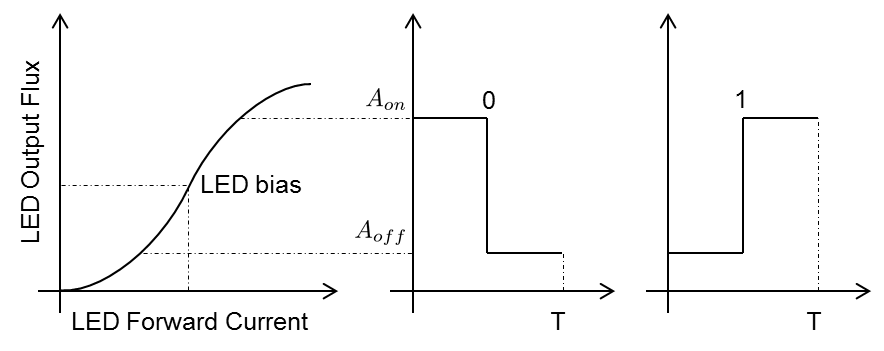
\includegraphics[trim={0in 0in 0in 0in}, clip=false, width=5.2in]{Signal_2PPM.png}
		\caption{2-PPM signals with 50$\%$ duty cycle.}
		\label{fig:sisoSig2PPM}
\end{figure}
%\subsection{Phase Shift Keying}
%\label{subsec:sisoModulationPSK}

\subsection{Optical Orthogonal Frequency Division Multiplexing}
\label{subsec:sisoModulationOOFDM}
OFDM is a spectrally efficient modulation technique and has been widely adopted for RF wireless communications. In OFDM, parallel streams of information are mapped over orthogonal frequency bins. Each bin is called a sub-carrier. Usually an $M$-ary QAM modulation is used to map information over each sub-carrier. An IFFT operation multiplexes the parallel streams to generate a time domain OFDM symbol to transmit. To mitigate interference due to multi-path, usually a CP is appended to the symbol before transmitting it. At the receiver, after removing the CP, an FFT operation demultiplexes the OFDM symbol to recover the parallel sub--carriers. Each sub-carrier is then demodulated to recover the information. OFDM has been successfully adapted and widely used for spectrally efficient OWC as summarized in reference \cite{arm09a}. For OWC, the time domain OFDM symbol is constrained to be real valued and unipolar. Ensuring Hermetian symmetry during symbol mapping over the orthogonal frequency bins will generate a real valued time domain signal. \figurename{ \ref{fig:sisoOOFDMBD}} illustrates signaling chain for O-OFDM. 

\afterpage{%
\clearpage
\begin{landscape}% Landscape page
\begin{figure}[t]
	\centering
		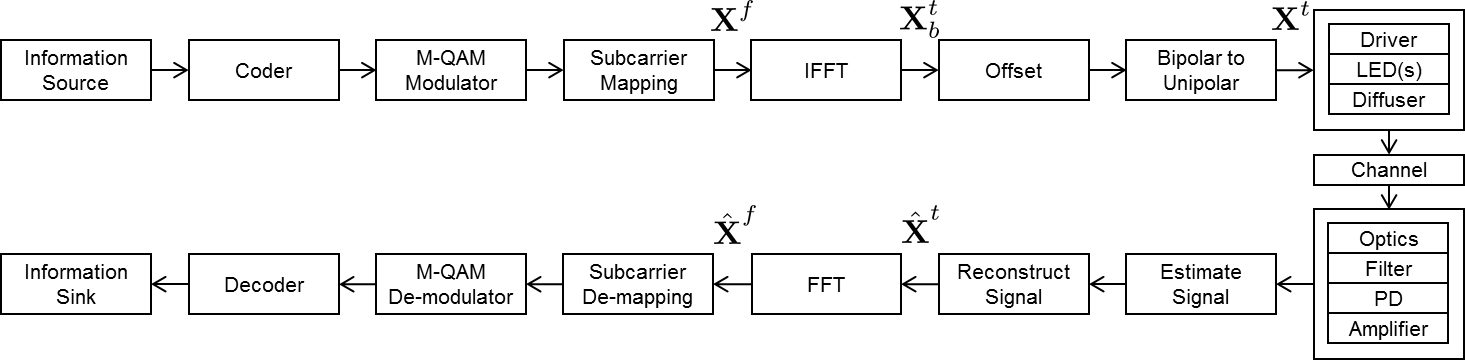
\includegraphics[trim={0in 0in 0in 0in}, clip=false, width=8in]{BlockDiagramOOFDM.png}
		\caption{O-OFDM Block Diagram.}
		\label{fig:sisoOOFDMBD}
\end{figure}
\end{landscape}
\clearpage% Flush page
}

Let $N_{sc}$ be the total number of sub-carriers for the O-OFDM frame. In DCO-OFDM,  the information bits are mapped to $N_{dco}^{d} = (N_{sc}/2) - 1$ number of data sub-carriers. An $M$-QAM modulator then assigns an $M$-QAM symbol corresponding the mapped bits on the data sub-carriers. The remaining sub-carriers are assigned Hermetian symmetric $M$-QAM symbols to form the frequency domain DCO-OFDM frame as shown in Eq.\eqref{eqDCOFrame}. 
\begin{equation}
	\vm{X}^{f} = [0; x_{1}^{ }; \ldots; x_{N_{dco}^{d}}^{ }; 0; x_{N_{dco}^{d}}^{*}; \ldots; x_{1}^{*}]
\label{eqDCOFrame}
\end{equation}

Taking an IFFT over frame $\vm{X}^{f}$ generates a bipolar time domain symbol $\vm{X}_{b}^{t}$. In DCO-OFDM the bipolar to unipolar conversion involves adding an offset to $\vm{X}_{b}^{t}$ such that majority of the the time domain symbol is non-negative and the symbol can then be clipped at zero. For relatively large $N_{sc}$, the signal values in the time domain are distributed normally. Thus adding an offset of at least 3.2$\times$SD ensures that less than 0.1$\%$ of signal values get clipped at zero - thus significantly reducing signal distortion due to clipping at the transmitter.

In ACO-OFDM, only the odd indexed sub-carriers carry data symbols. Hermetian symmetry is then enforced to obtain real valued time domain symbol. The information bits are mapped to $N_{aco}^{d} = (N_{sc}/4)$ number of data sub-carriers. An $M$-QAM modulator then assigns an $M$-QAM symbol corresponding the mapped bits on the data sub-carriers. The frequency domain ACO-OFDM frame construction is shown in Eq.\eqref{eqACOFrame}. 
\begin{equation}
	\vm{X}^{f} = [0; x_{1}^{ }; 0; x_{2}; \ldots; x_{N_{aco}^{d}}^{ }; 0; x_{N_{aco}^{d}}^{*}; \ldots; 0; x_{2}^{*}; 0; x_{1}^{*}]
\label{eqACOFrame}
\end{equation}

Taking an IFFT over frame $\vm{X}^{f}$ generates a bipolar time domain symbol $\vm{X}_{b}^{t}$. In ACO-OFDM bipolar to unipolar conversion is achieved by simply clipping the symbol at zero. It has been shown in reference \cite{arm06a} that this clipping introduces noise only on the non-data bearing even indexed sub-carriers. Thus by simple signal processing, an estimate of transmitted signal can be reconstructed. The $N_{aco}^{d}$ data sub-carriers are then demodulated and decoded to recover transmitted information. Implementation and performance comparisons of ACO-OFDM and DCO-OFDM is shown in reference \cite{mes11a}.
